\chapter{Research Methods}
\lhead{\emph{Research Methods}}

This chapter provides information about the research methods used in this project. Before conducting a series of experiments, to explore and evaluate machine learning methods, it was needed to decide on how are these algorithms going to be implemented and evaluated. Choices of a programming language,  a machine learning library, and an evaluation method are explained in this chapter.

\section{Choice of a Programming Language}

 It was chosen to use Python programming language for implementing this project. The language was chosen because it is one of the most popular languages used by machine learning researchers and developers. It is also free and open source. Since Python is an interpreted language, code written in Python can be executed on multiple different platforms without having a need to modify the code. Beacuse  Python is a very popular language, there are many publicly available  open source packages with efficient implementation of machine learning algorithms for this language.

Availability of scientific computing tools for Python was also one of the main reasons why this language was chosen. Scientific Python libraries that were used in this project were Matplotlib, NumPy, IPython and Jupyter Notebook \citep{scipy}. Matplotlib provided an ability to plot graphs, images, and tables. NumPy was used for efficient arithmetical operations with matrices. IPython allowed to execute only a part of a program without a need to run a full code. It is a system for an interactive scientific computing \citep{ipython}. Some of the operations, for example, loading the dataset or resizing the images can take a long time to complete. In IPython these operations is only required to be completed once. Then, results of these operations are saved in memory where they remain and can be reused. Jupyter Notebook allowed to execute Python code in a web browser and  save the results as HTML pages \autoref{fig:jupyter}. Jupyter Notebook is an IPython wrapper that launches a HTTP server. Scientific Python libraries allowed to interactively explore the data with an  ability to plot graphs, tables and visualize  results.

The alternative language that was also considered was Matlab. Matlab is a domain specific programming language that was designed specifically for matrix programming. It also includes an image processing and machine learning toolboxes. Machine learning and image processing functions are easier to use in Matlab than in Python, because this language was developed for a particular purpose. However, Matlab is a closed source language. It also only supports some platforms, where Python code can be executed in almost any computing environment. Therefore, Python programming language was a better option.

\begin{figure}[ht]
\centering
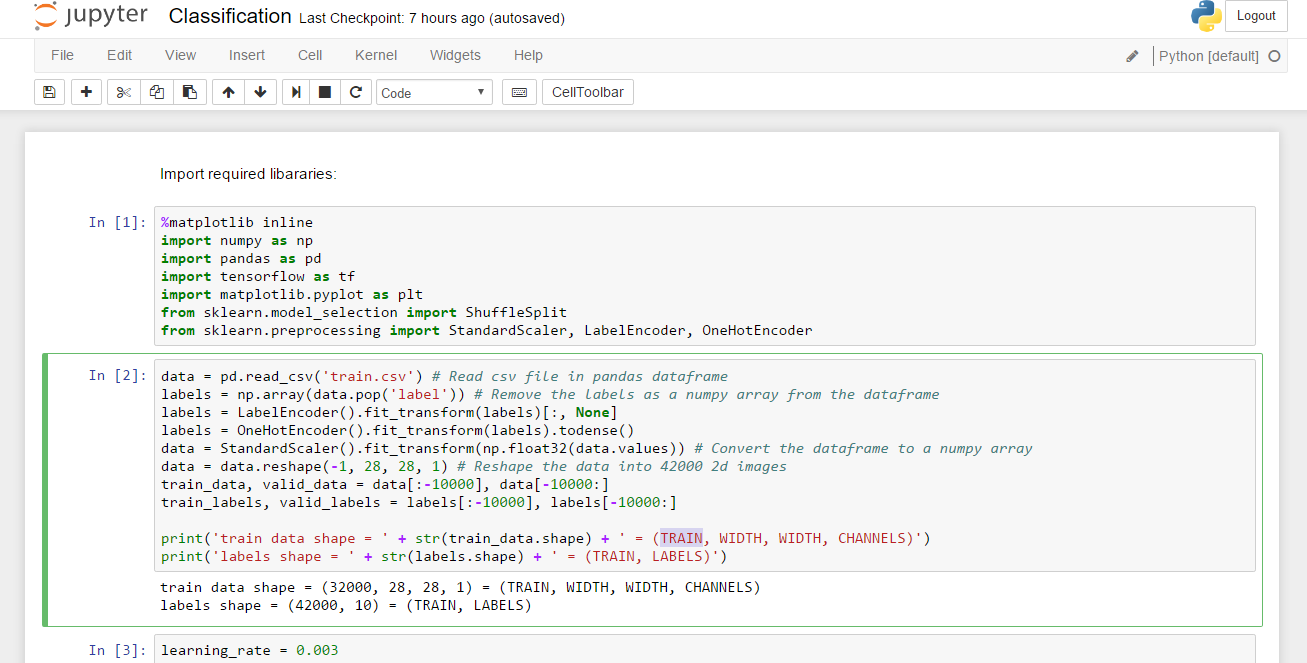
\includegraphics[width=14cm]{Figures/c3/c3jupyter.PNG}
\caption{Example of a Jupyter Notebook}
\label{fig:jupyter}
\end{figure}


\section{Choice of Machine learning libraries}

\subsection{Why was a Machine Learning Library Needed?}

It is possible to implement machine learning algorithms without using any additional library. However, there are many benefits provided by machine learning libraries. Algorithms available in machine learning libraries  are often implemented more efficiently. Adapting a provided algorithm for a specific task also takes a less time  than  writing a particular algorithm for it. Therefore, it was decided to analyse what machine learning libraries  are available for Python.

\subsection{Library Used for Machine Learning }

Sckit-learn python package was chosen as a library for working with machine learning models. This package provides state-of-the-art implementations of many well-known machine learning algorithms and has an easy-to-use interface tightly integrated with the Python language \citep{pedregosa2011scikit}. Large parts of this module are written in C or C++. Because C and C++ are much faster than Python, it makes algorithms run faster compared to a standard Python implementation. Sckit\-learn machine learning algorithms are high-level API's \citep{buitinck2013api}. Algorithms provided in this package do not require a knowledge of their implementation details. Nevertheless, Sckit-learn interface allow parameters of these algorithms to be configured.

In the case of food image classification, the main advantages that Sckit-learn provided were the fact that it uses the same data input format for every machine learning algorithm and ability to easily configure parameters, to make classifiers work on image classification.


\section{The Evaluation Method for the Classification Algorithms}

The key indicator of performance in the classification task is a classification accuracy. Accuracy is calculated by dividing the number of correct predictions by the total number of predictions. By calculating and comparing accuracy scores for every machine learning algorithm tried, the best food image classification technique was found.

Other helpful performance indicators used to evaluate a classification performance when parameters of classification algorithms were tuned were: confusion matrix, precision, recall and f measure. Confusion matrix shows how often and what classes are misclassified as other classes. Precision is the total number of elements classified correctly divided by a total number of elements that were classified as that class. A recall is the total number of items classified correctly divided by a total number of items of that type in the database. A graphical illustration of precision and recall measures is shown in \autoref{fig:p}.  F-measure is a measure combined from precision and recall according to a formula \( F = 2 \frac{Recall \times Precision }{Recall  +  Precision} \)   \citep{ting2011}. 


\begin{figure}[ht]
\centering
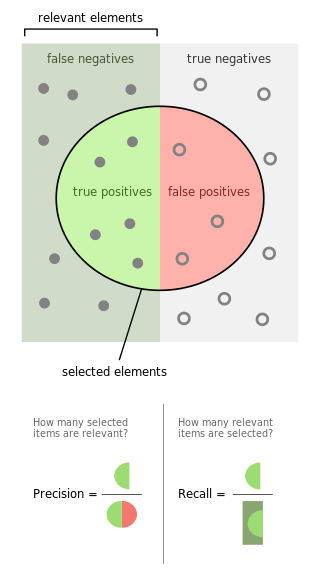
\includegraphics[width=5cm]{Figures/c3/p.png}
\caption{Graphical illustration of the precision and recall \cite{wiki:p}}
\label{fig:p}
\end{figure}


\section{Summary}
In this chapter reasoning behind a chosen programming language and machine learning library used was provided. Methods for evaluating the performance of classification algorithms were discussed. Accuracy score was picked as the primary method for performance evaluation. In the following chapter, accumulation of a food image dataset is discussed.